\documentclass{article}
\usepackage[letterpaper]{geometry}
\geometry{verbose,tmargin=1in,bmargin=1in,lmargin=1in,rmargin=1in}

\usepackage[utf8]{inputenc}
\usepackage{amsmath}
\usepackage{float}
\usepackage{listings}
\usepackage{graphicx}
\usepackage{enumitem}

\renewcommand{\baselinestretch}{1.5}

\title{CIS 419/519: Homework 5}
\author{\{Yupeng Li\}}
\date{03.17.2020}

\begin{document}
    \maketitle
    Although the solutions are entirely my own, I consulted with the following people and sources while working on this homework: \textbf{https://www.youtube.com/watch?v=kNPGXgzxoHw}
    \paragraph{PART I: PROBELM SET}
    \section{Logical Functions with Neural Nets}
    \textbf{(a)} 
    The NAND logic follows a truth table as follows:
    \begin{center}
\begin{tabular}{ c c c }
 $x_0$ & $x_1$ & $H(x)$ \\ 
 0 & 0 & 1 \\  
 0 & 1 & 1 \\  
 1 & 0 & 1 \\
 1 & 1& 0  \\
\end{tabular}
\end{center}

If we use sigmoid as our activation function at the output node, where $\sigma(z) = \frac{1}{1+exp(-z)}$
\\and $H(x) = \sigma(w_0 + w_1 x_0 + w_2 x_2)$, where $w_0 = 40$, and $w_1 = w_2 =  -25$ we would then have:

\begin{center}
\begin{tabular}{ c c c }
 $x_0$ & $x_1$ & $H(x)$\\ 
 0 & 0 & $\sigma(40) = 1$ \\  
 0 & 1 & $ \sigma(15) = 1$ \\  
 1 & 0 & $\sigma(15) = 1 $\\
 1 & 1 & $ \sigma(-10) = 0$
\end{tabular}
\end{center}
The neural network that is used to compute this function is the same as in the graph given in the problem set. 

		\begin{figure}[H]
			\caption{Neural network for NAND Logic}
			\centering
			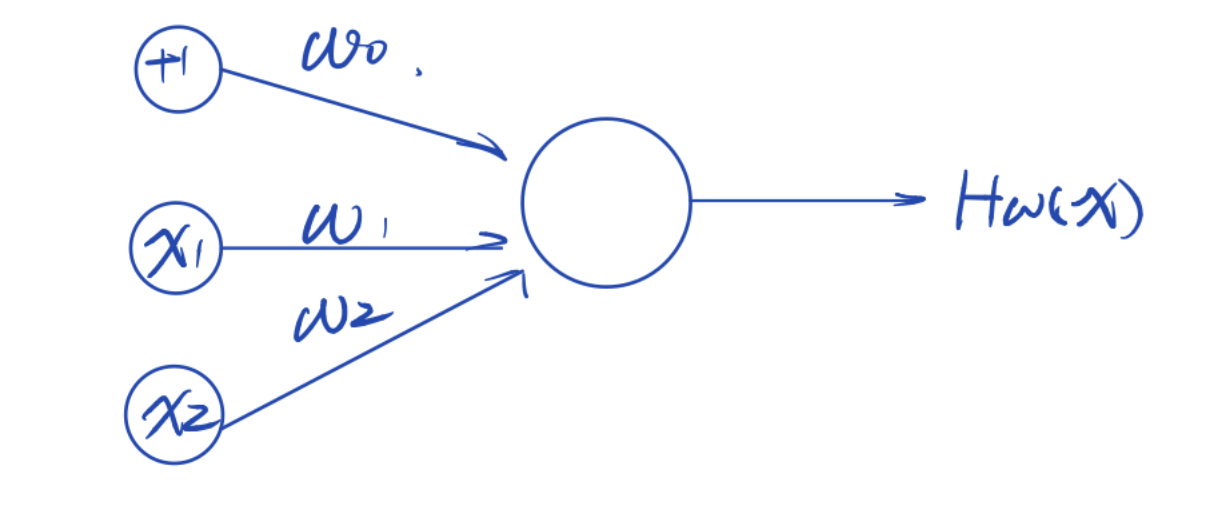
\includegraphics[width=8cm]{HW5_1.jpeg}
		\end{figure}

\textbf{(b)} The parity of three binary inputs follows a truth table as in the table underneath:
\begin{center}
\begin{tabular}{ c c c c }
 $x_0$ & $x_1$ & $x_2$ & $H(x)$ \\ 
 1 &0 & 0 & 1 \\  
 0 &0 & 1 & 1 \\  
 0 &1 & 0 & 1 \\
 0 &1 & 1& 0  \\
 1&1&0&0\\
 1&0&1&0\\
 0&0&0&0\\
 1&1&1&1\\
\end{tabular}
\end{center}
The parity of three binary inputs can be characterized by two consecutive XOR gates. Neural network for the parity is demonstrated in the following figure:
		\begin{figure}[H]
			\caption{Neural network for parity Logic}
			\centering
			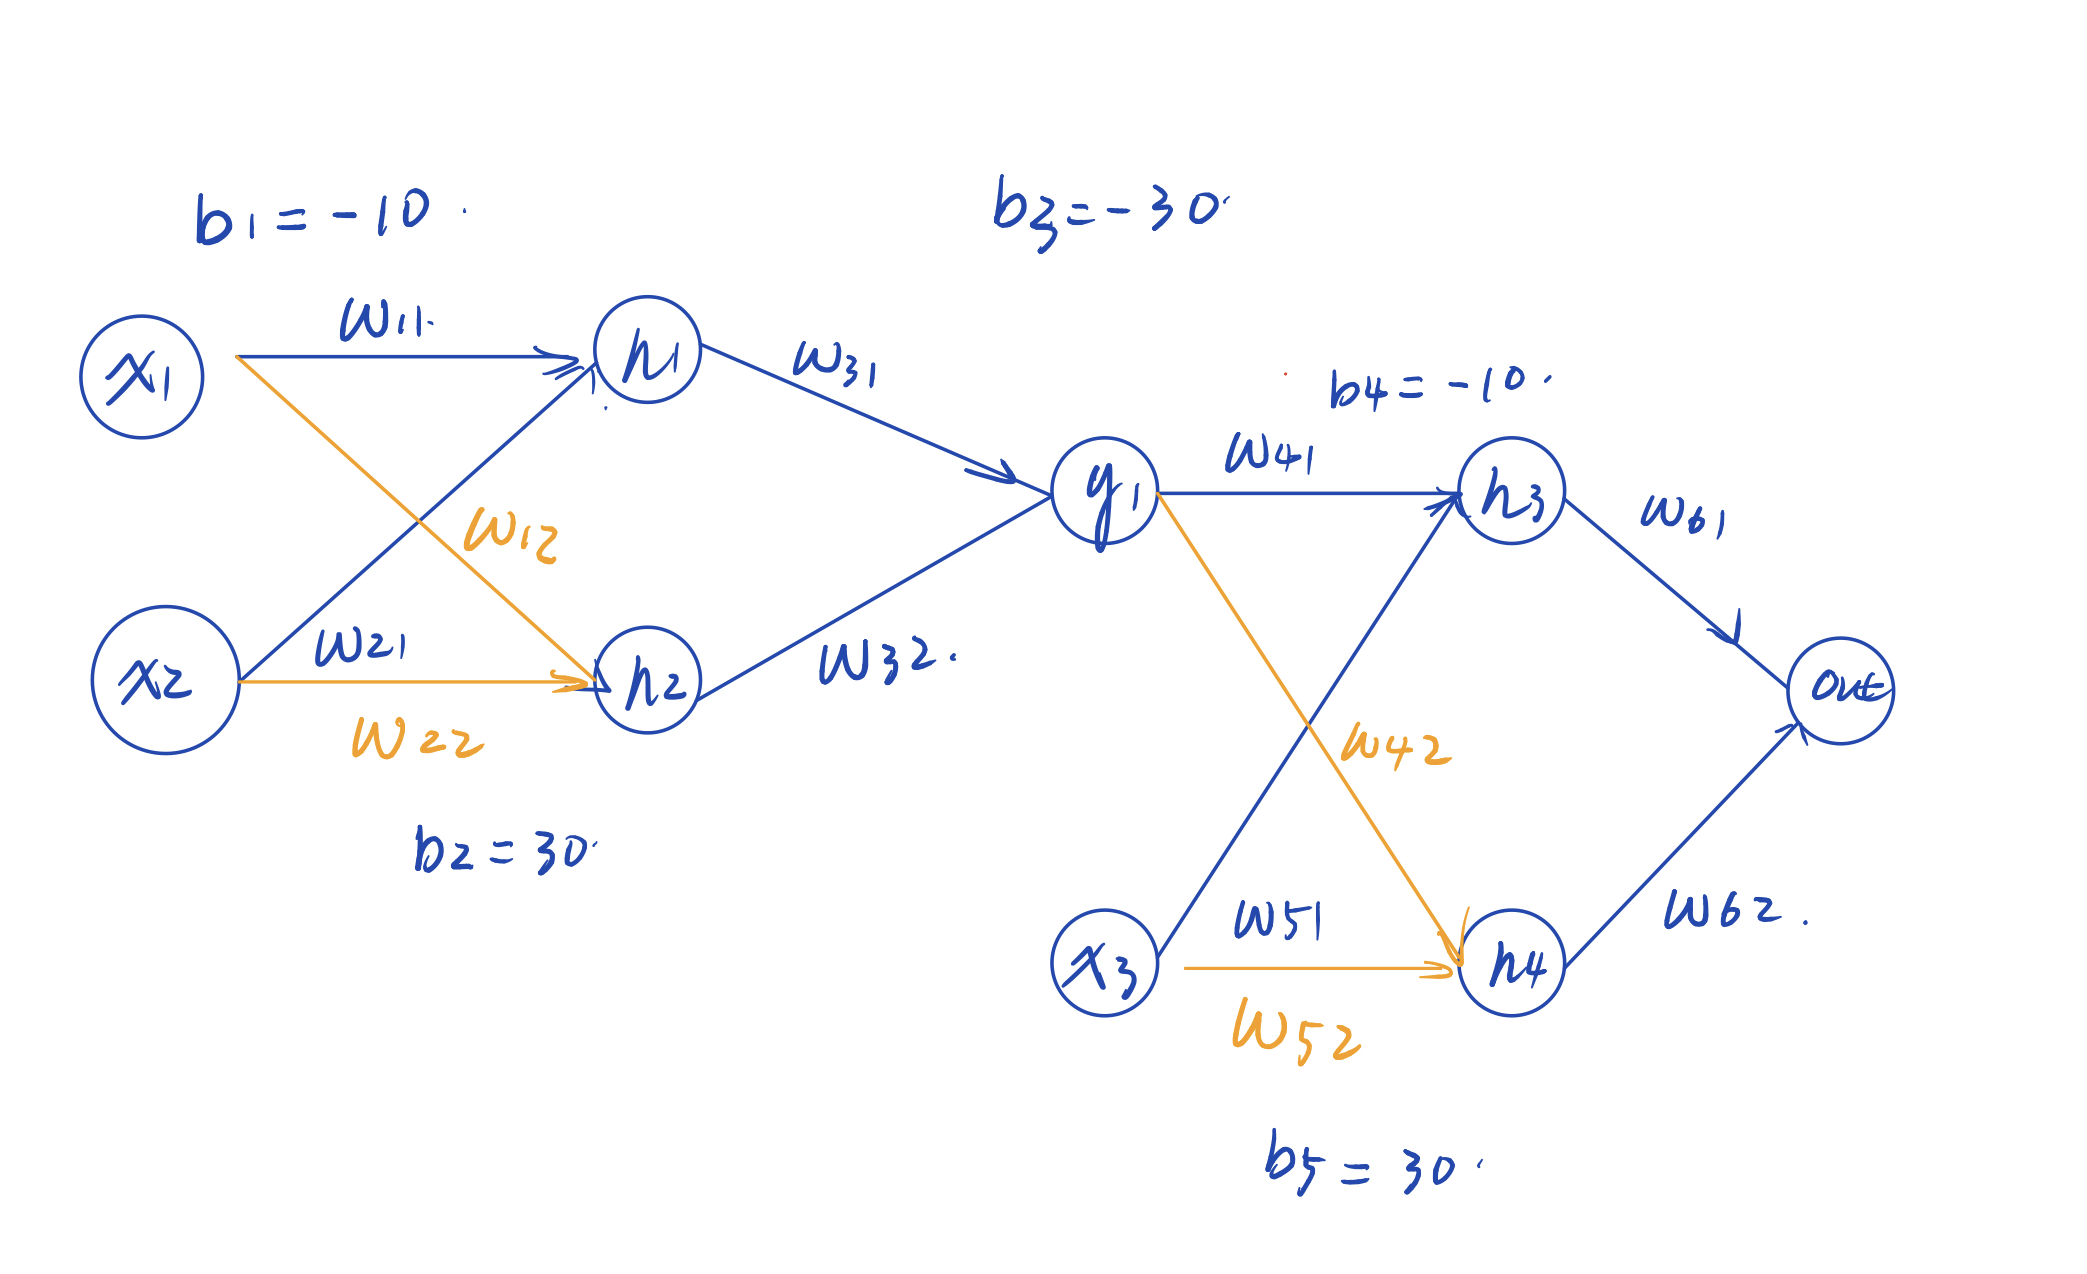
\includegraphics[width=8cm]{1_b.jpeg}
		\end{figure}
As in the figure, the weights are \[w_{11} = w_{21} = w_{41} = w_{51} =20\]
\[w_{12}=w_{22} = w_{42} = w_{52} = -20\]
\[w_{31} = w_{32} = w_{61} = w_{62} = 20\]
\[b_{1} = b_{4} = -10\]
\[b_{2} = b_{5} = 30\]
    
Sigmoid is applied as activation function in each hidden layer. Thus the left half can easily be proved to have XOR logic. Combining two XOR gates we can easily get the truth table as above.
\\For this section of homework, I referred to \textbf{https://www.youtube.com/watch?v=kNPGXgzxoHw}

\section{Calculating Backprop by Hand}
We can first calculate the hidden layer using the following equation:
\begin{align}
Sign(
\begin{bmatrix}
0.1 & 0.2 \\
-0.4 & 0.3
\end{bmatrix}
\begin{bmatrix}
5\\
4
\end{bmatrix}
)
=
H
\end{align}
Thus,
\begin{align}
H  = 
\begin{bmatrix}
1\\
-1
\end{bmatrix}
\end{align}
The output is then
\begin{align}
\sigma(
\begin{bmatrix}
0.1 & 0.2
\end{bmatrix}
\begin{bmatrix}
1\\
-1
\end{bmatrix}
) =0.524979
\end{align}
The final output can be written in the form
\[Output = \sigma(1\cdot W_{1}^{2}-1\cdot W_{2}^{2})=\frac{1}{1+e^{-(1\cdot W_{1}^{2}-1\cdot W_{2}^{2})}}\]
Thus,
\[Output = \frac{1}{1+e^{W_{2}^{2}-W_{1}^{2}}}\]
Taking partial derivative with respect to $W_{2}^{1}$ and $W_{2}^{2}$ respectively, we can easily obtain the gradient matrix between the hidden layer and output layer which is:
\begin{align}
h = 
\begin{bmatrix}
0.249376\\
-0.249376
\end{bmatrix}
\end{align}

For the gradient with respect to the input layer:
\begin{align}
W^{1} =
\begin{bmatrix}
0.1 & 0.2\\
-0.4 & 0.3
\end{bmatrix}
\end{align}
The gradient of the output with respect to the top left weight $W_{11}^{1}$ is just:
\[\frac{\partial{h(1)}}{\partial{W_{11}^{1}}} \times \frac{\partial{Output}}{\partial{h(1)}}\]
\\Based on calculations:
\[ \frac{\partial{Output}}{\partial{h(1)}} = 0.0249376 \]
\[\frac{\partial{h(1)}}{\partial{W_{11}^{1}}} = 5 \cdot \nabla Sign(1) = 5\]  
Thus the output gradient with respect to  $W_{11}^{1}$ is just 0.124688
\\Following similar reasoning, the gradient between the output and the first layer weight can be constructed as in the following matrix:
\begin{align}
\begin{bmatrix}
0.124688 & 0.249376\\
0.0997504 & 0.199501
\end{bmatrix}
\end{align}
    \paragraph{PART II: PROGRAMMING EXERCISES}
    
    All of part 2 are submitted  in HW5.ipynb and cnn.th
\end{document}